
\section{The Transfer Function}


\begin{frame}
\frametitle{The transfer function}

From previous lectures:
\begin{align*}
    y(t) &= h(t) \otimes u(t)  \\
    \Rightarrow \quad 
    \mathscr{L}\{y(t)\} &= \mathscr{L}\{h(t) \otimes u(t)\}  \\
    \Rightarrow \quad
    Y(s) &= H(s) \cdot U(s)\\
    H(s) &= \frac{Y(s)}{U(s)}
\end{align*}
This is the transfer function, the relation between input and output in the Laplace domain (continuous time systems)


\end{frame}

\begin{frame}
\frametitle{Plot of H(s)?}

\begin{itemize}
\item $s$ and $H(s)$ are both complex $\rightarrow$ 4D-graph?
\item No, we will substitute $s$ for $j\omega$ with $\omega$ the angular frequency [rad/s].
(We will often use frequency to indicate $\omega$ but keep in mind that $\omega = 2\pi f)$
\item We will also split $H(s) = H(j\omega)$ using its polar representation in two, an amplitude and a phase plot
\item Remember: $H(j\omega) = |H(j\omega)| \exp\angle(H(j\omega))$ 
\item The amplitude plot and the phase plot of $H(j\omega)$ are called the bode plot

\end{itemize}
\end{frame}


\section{What Is The Bode Plot}

\begin{frame}
\frametitle{The amplitude plot}

Convention: 
\begin{itemize}
\item for the ordinate (y-axis) we use $20\log_{10}|H(j\omega)|$ with the special unit $dB$
\item for the abscissa (x-axis) we use a logarithmic plot of $\omega$

\end{itemize}
This is thus a bi-log plot

The reason for using the logarithm of the modulus of $H(j\omega)$ will become clear later

\end{frame}




\begin{frame}
\frametitle{The phase plot}
Convention:
\begin{itemize}
\item for the ordinate (y-axis) we use $\angle H(j\omega)$ in degrees
\item for the abscissa (x-axis) we use a logarithmic plot of $\omega$

\end{itemize}
This is thus a semi-log plot


\end{frame}


\begin{frame}
\frametitle{Example bode plot}
$H(s) = \frac{14s^2 + 7s + 3}{s^4 + 10s^3 + 10s^2 + 10s + 10}$
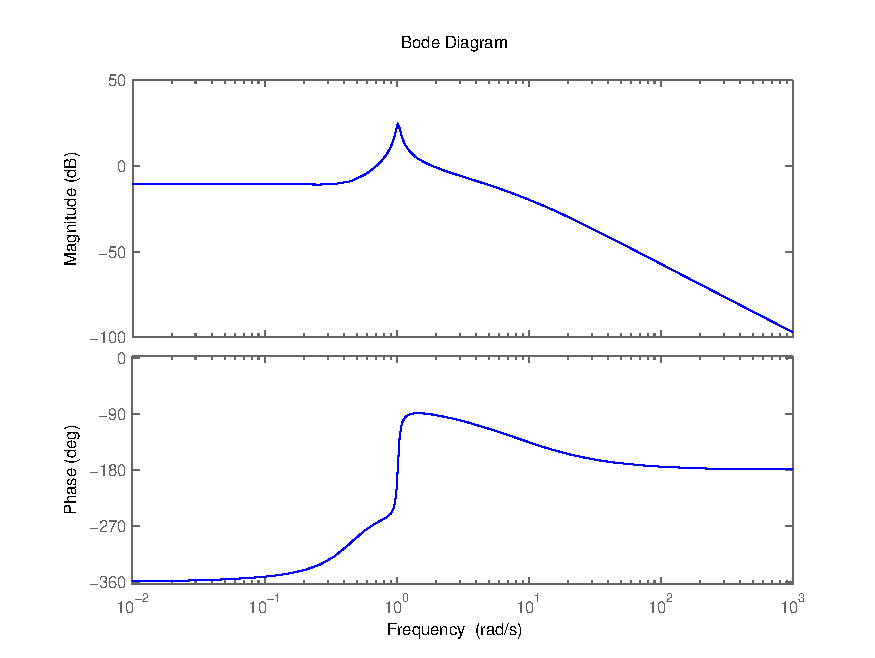
\includegraphics[scale=0.5]{ExampleBode1}


\end{frame}


\section{How To Construct A Bode Plot (by hand)}

\begin{frame}
\frametitle{A new representation of the transfer function}
From before:
\begin{align*}
H(s) &= \frac{\beta_0 s^r + \beta_1 s^{r-1} + \ldots + \beta_r}{s^n + \alpha_1 s^{n-1} + \ldots + \alpha_n}\\
\text{Factorization in zeros and poles}\\
\Rightarrow \quad
H(s) &= \frac{\beta_0 (s-n_1) (s-n_2) \ldots (s-n_r)}{(s-p_1) (s-p_2) \ldots (s-p_n)}
\end{align*}
This is the usual representation. Now however, we will look for factors $(1+\displaystyle{\frac{s}{s_i}})$, with $s_i$ a so-called breakpoint.


\end{frame}


\begin{frame}
\frametitle{A new representation of the transfer function}
We can do this by bringing all the zeros and poles not equal to zero outside the brackets, as follows:
$$H(s) = \beta_0 \frac{\prod(-n_i)}{\prod(-p_j)} \frac{(1+\frac{s}{-n_1}) (1+\frac{s}{-n_2}) \ldots (1+\frac{s}{-n_i})}{s^l (1+\frac{s}{-p_1}) (1+\frac{s}{-p_2}) \ldots (1 + \frac{s}{-p_j})}$$
 Replacing the constants by $K$, and setting $$r_k = -n_k$$ $$ s_k = -p_k$$ 



\end{frame}



\begin{frame}
\frametitle{A new representation of the transfer function}

We ultimately get: $$H(s) = K \frac{(1+\frac{s}{r_1}) (1+\frac{s}{r_2}) \ldots (1+\frac{s}{r_i})}{s^l (1+\frac{s}{s_1}) (1+\frac{s}{s_2}) \ldots (1 + \frac{s}{s_j})}$$
Now we are able to construct the bode plot of each different factor of $H(s)$. Afterwards we can just add up these plots using the calculation rules of complex numbers.

  
\end{frame}



\begin{frame}
\frametitle{Intermezzo complex numbers}
\begin{itemize}
\item The amplitude of the product of complex numbers is equal to the product of the amplitudes of these numbers
\item The phase of the product of complex numbers is equal to the sum of the phases of these numbers
\item The logarithm of a product of numbers is equal to the sum of the logarithms of these numbers

\end{itemize}
This comes down to 
$$ 20\log_{10}|H(j\omega)| = \sum 20\log_{10}|\text{factors}| $$ 
$$ \angle H(j\omega) = \sum(\angle \text{factors})$$

Next we will quickly go over the simple bodeplots of the different factors of $H(s)$

\end{frame}



\begin{frame}
\frametitle{The constant K}
\begin{itemize}
\item $20\log_{10}|K| =$ constant
\item $\angle K = 0^{\circ} \text{ or} \pm 180^{\circ}$  (resp $K > 0$ and $K < 0$)
\end{itemize}
Example: $K = 10$
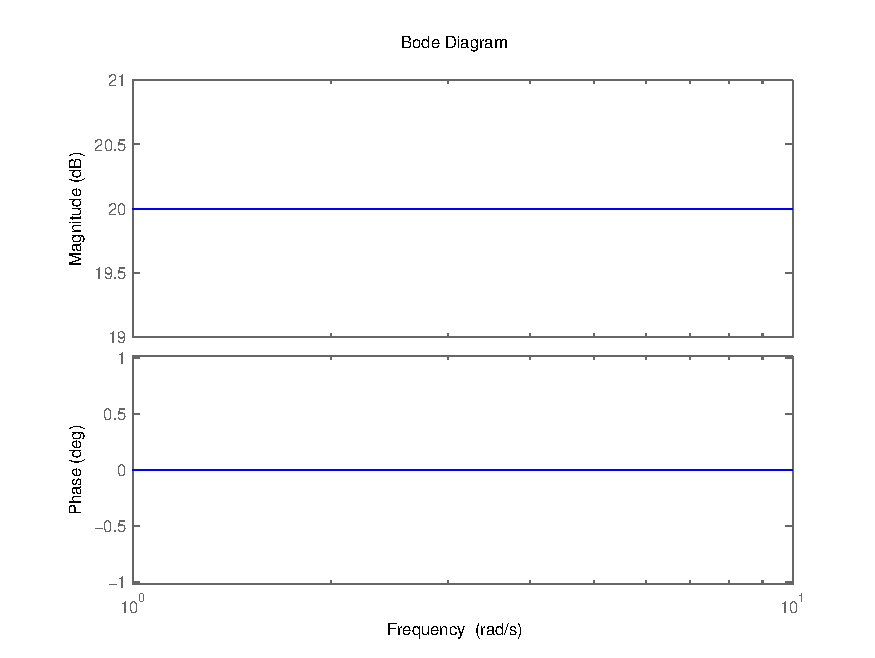
\includegraphics[scale=0.5]{BodeConstant}

\end{frame}



\begin{frame}
\frametitle{$(1+\frac{j\omega}{r_i})$ in the numerator}
(Assume $r_i > 0$)
\begin{itemize}
\item What if $\omega \rightarrow 0$ ? \quad $(1+\frac{j\omega}{r_i}) \rightarrow 1$
\begin{itemize}
\item $20\log_{10}|1| = 0$
\item $\angle 1 = 0^{\circ}$
\end{itemize}

\item What if $\omega \rightarrow \infty$ ?  \quad  $(1+\frac{j\omega}{r_i}) \rightarrow j\infty$
\begin{itemize}
\item $20\log_{10}|j\infty| = \infty$
\item $\angle j\infty = 90^{\circ}$
\end{itemize}

\item The two terms balance each other out for $\omega = r_i$ (remember, this is called a break point).
\begin{itemize}
\item $20\log_{10}|1+j| = 20\log_{10}(\sqrt 2) \approx 3 \text{dB}$
\item $\angle(1+j) = 45^{\circ}$
\end{itemize}
\end{itemize}
A break point is therefore also called a 3dB point
\end{frame}



\begin{frame}
\frametitle{$(1+\frac{j\omega}{r_i})$ in the numerator}
Example: $r_i = 100$
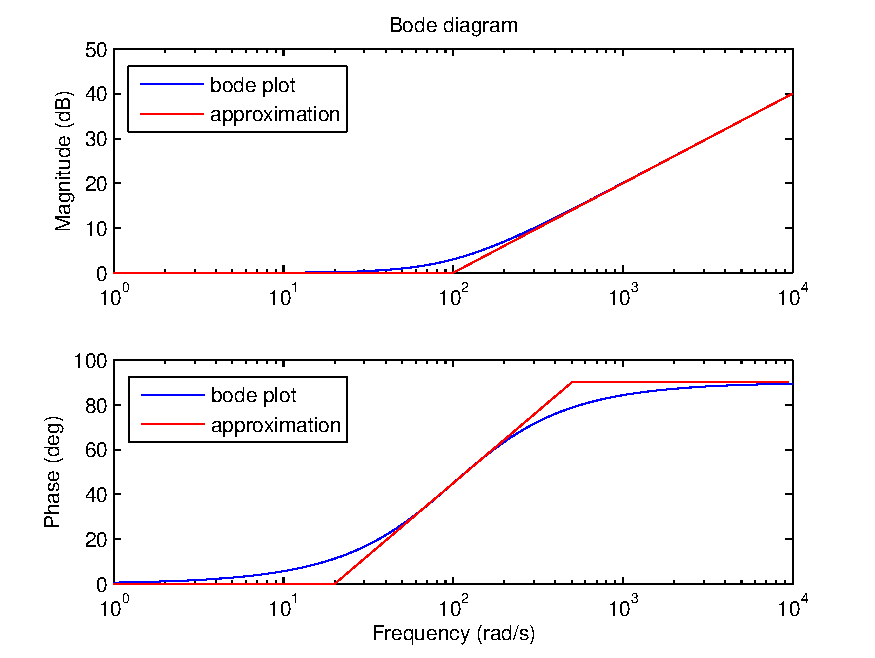
\includegraphics[scale=0.5]{BodeNumerator}

\end{frame}



\begin{frame}
\frametitle{$(1+\frac{j\omega}{s_i})$ in the denominator}
This factor is equivalent to the previous one. The only difference is the sign change in both plots as:
\begin{itemize}
\item $\log |\frac{1}{z}| = -\log|z|$
\item $\angle \frac{1}{z} = -\angle z$
\end{itemize}


\end{frame}


\begin{frame}
\frametitle{$(1+\frac{j\omega}{s_i})$ in the denominator}

%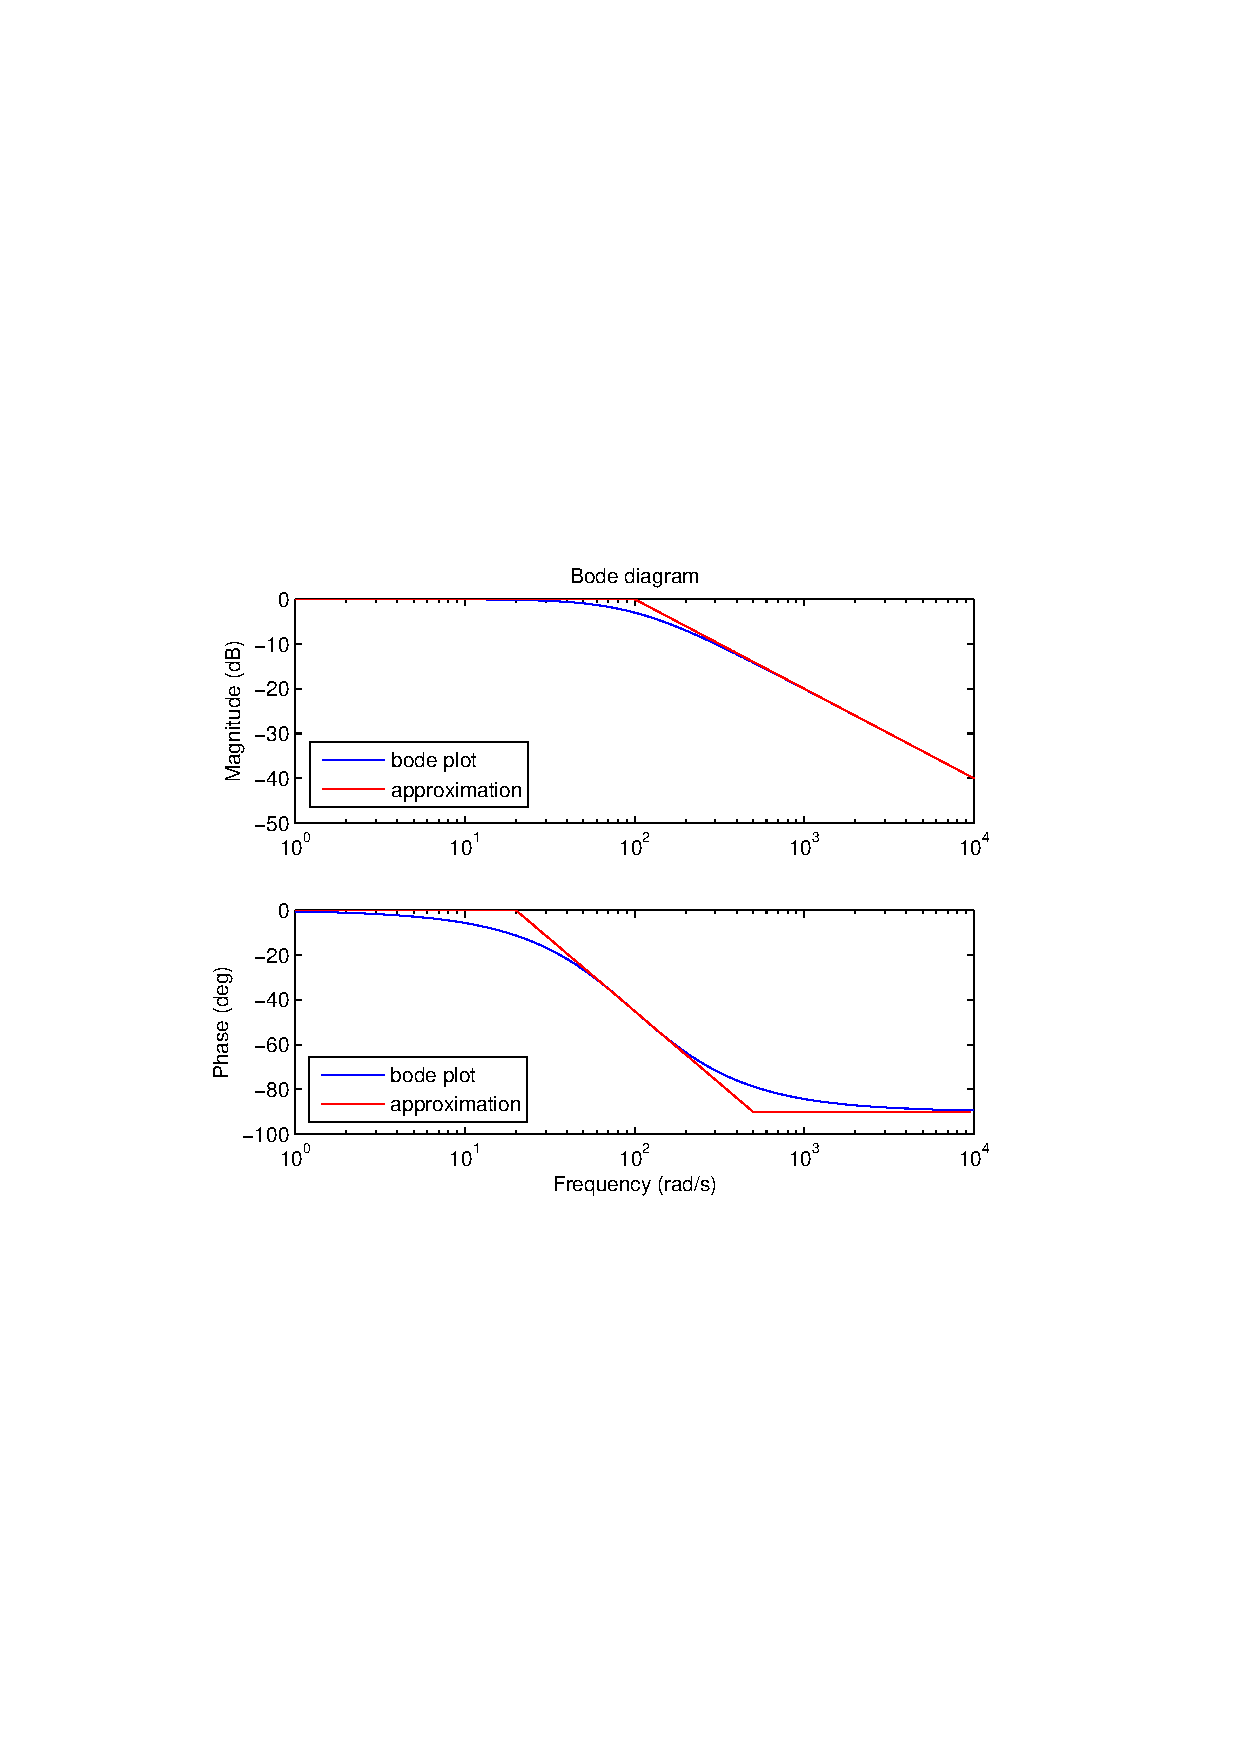
\includegraphics[scale=0.5]{BodeDenominator}


\end{frame}


\begin{frame}
\frametitle{$j\omega$ in the numerator}
\begin{itemize}
\item This is simply a (ascending) straight line in the amplitude plot, with a slope of 20 dB/decade
\item Constant phase of $90^{\circ}$
\end{itemize}

%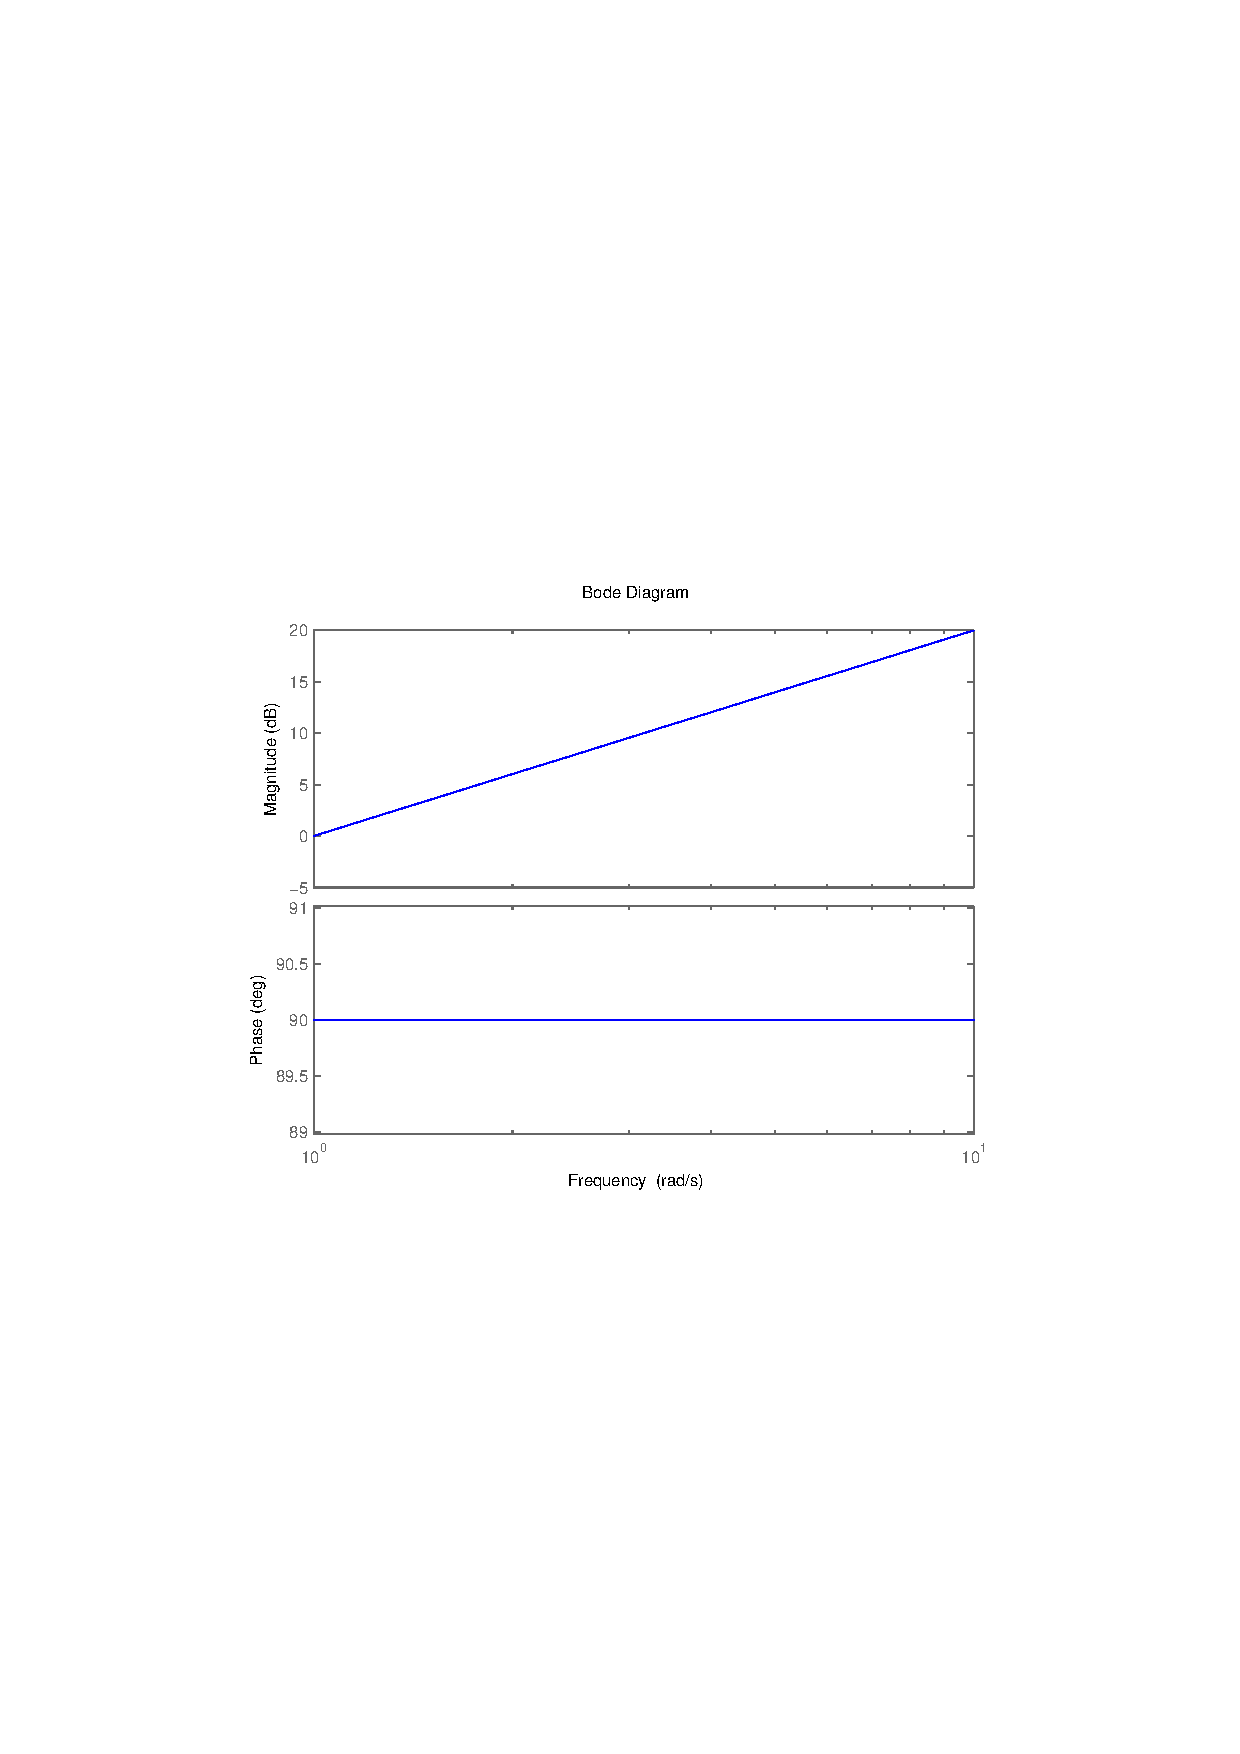
\includegraphics[scale=0.5]{BodeZeroNum}

\end{frame}



\begin{frame}
\frametitle{$j\omega$ in the denominator}

\begin{itemize}
\item This is simply a (descending) straight line in the amplitude plot, with a slope of -20 dB/decade
\item Constant phase of $-90^{\circ}$
\end{itemize}

%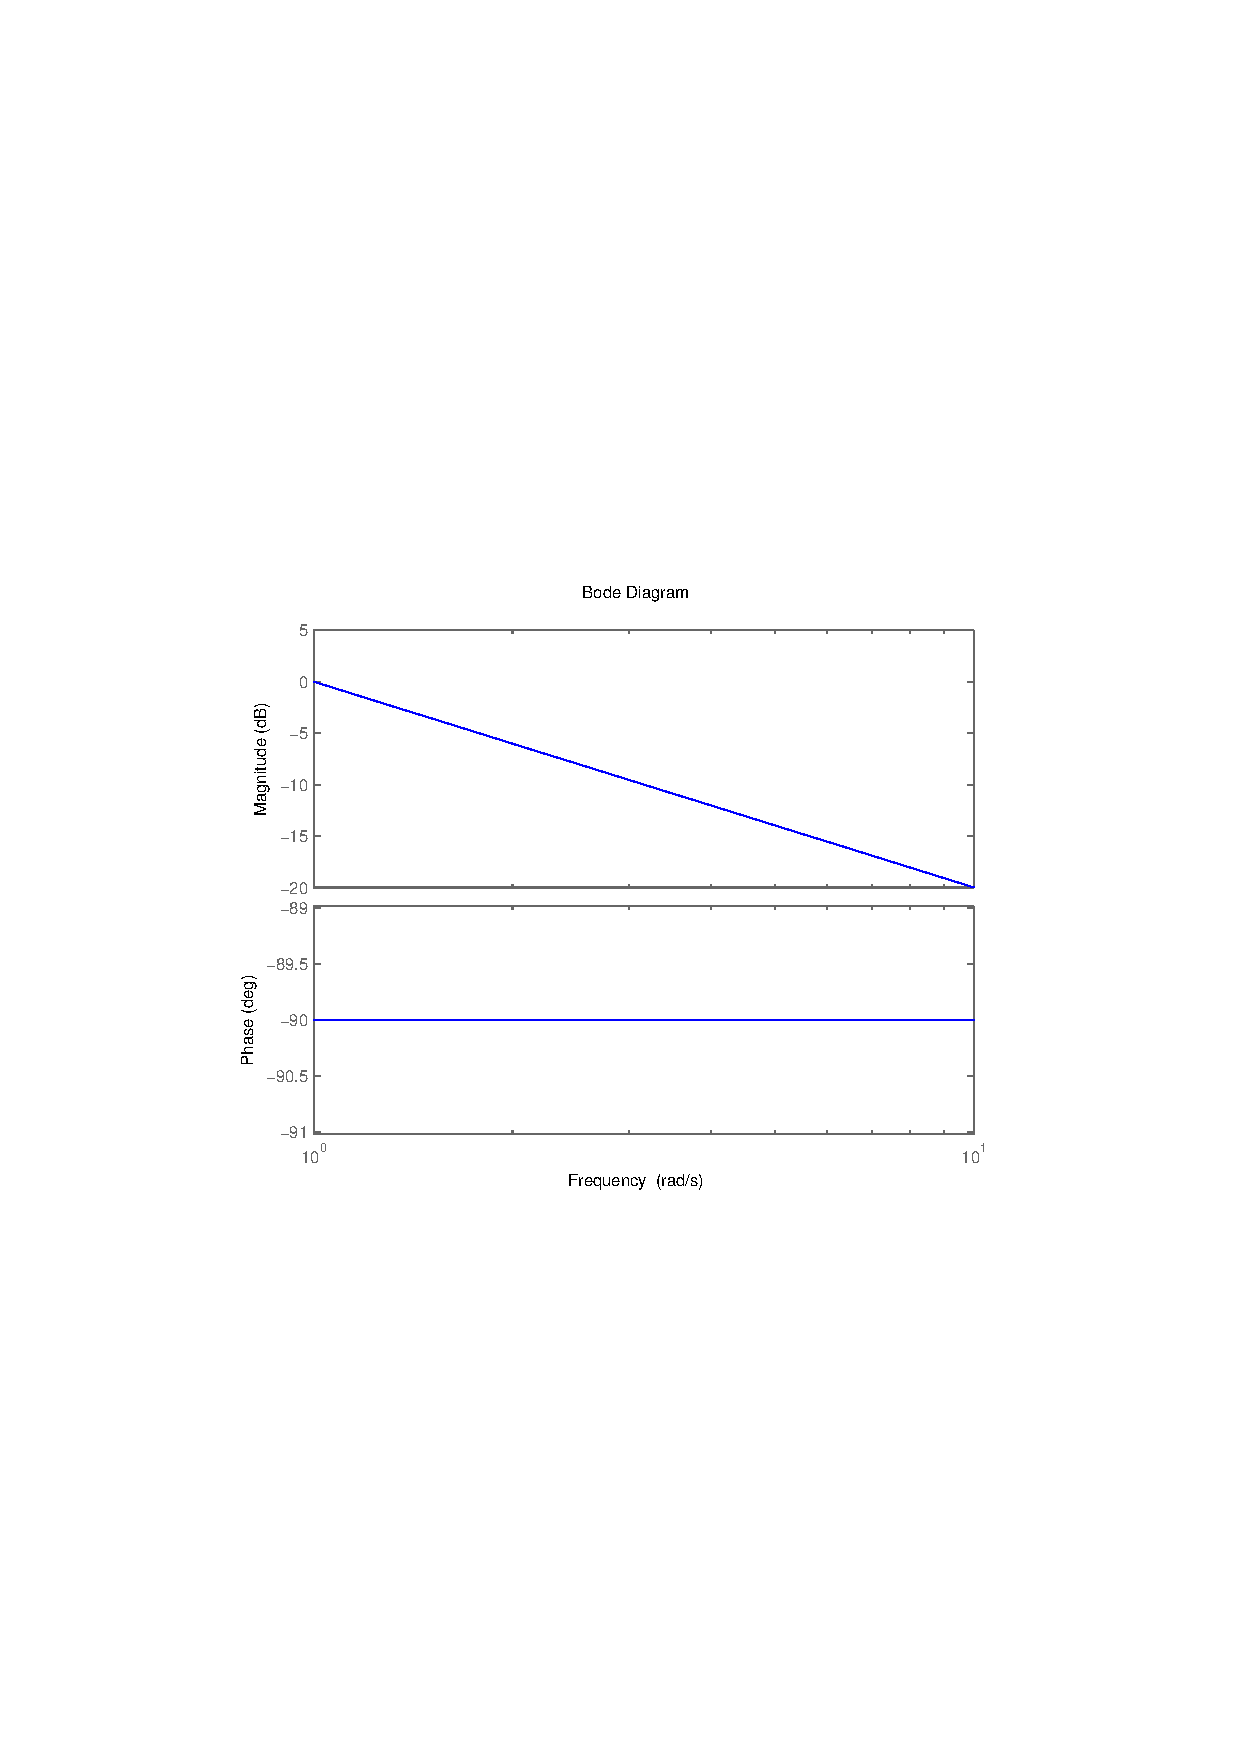
\includegraphics[scale=0.5]{BodeZeroDen}


\end{frame}



\begin{frame}
\frametitle{Second order factors}
A second order factor has twice the effect of a first order factor.\\
Consider for example $(1+\frac{j\omega}{100})^2$ in the numerator:

%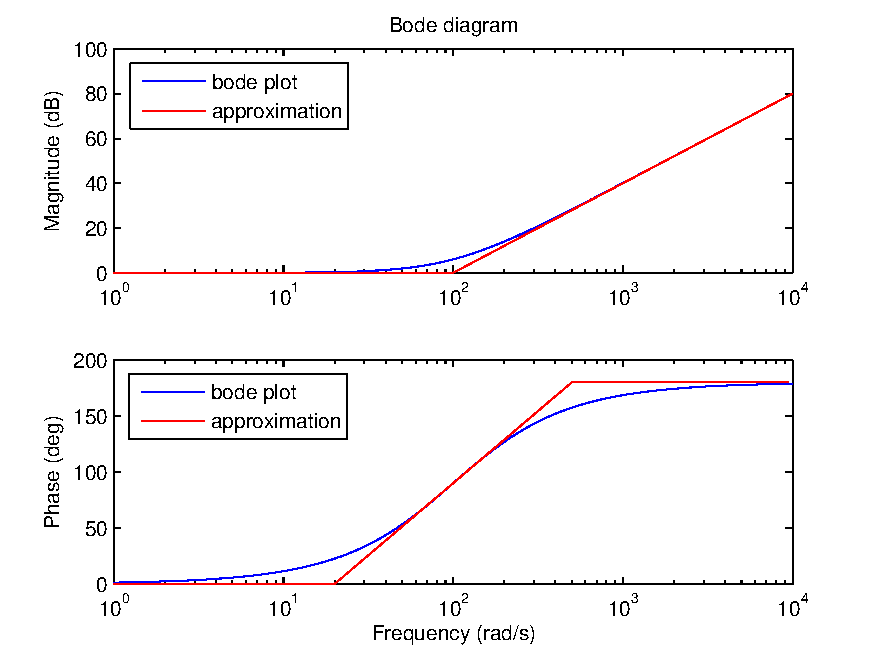
\includegraphics[scale=0.5]{BodeSecondOrder}

Similar for higher order factors

\end{frame}


\begin{frame}
\frametitle{Exception}
Up until now we always considered $r_i \text{ and } s_i > 0$, but what if we had a factor $(1-\frac{j\omega}{r_i})$ for example?
\begin{itemize}
\item The amplitude plot remains unchanged, as $|1+\frac{j\omega}{r_i}| = |1 - \frac{j\omega}{r_i} |$
\item The phase plot is reversed, as $\angle(1+\frac{j\omega}{r_i}) = -\angle(1 - \frac{j\omega}{r_i})$
\end{itemize}



\end{frame}


\begin{frame}
\frametitle{Exception}

%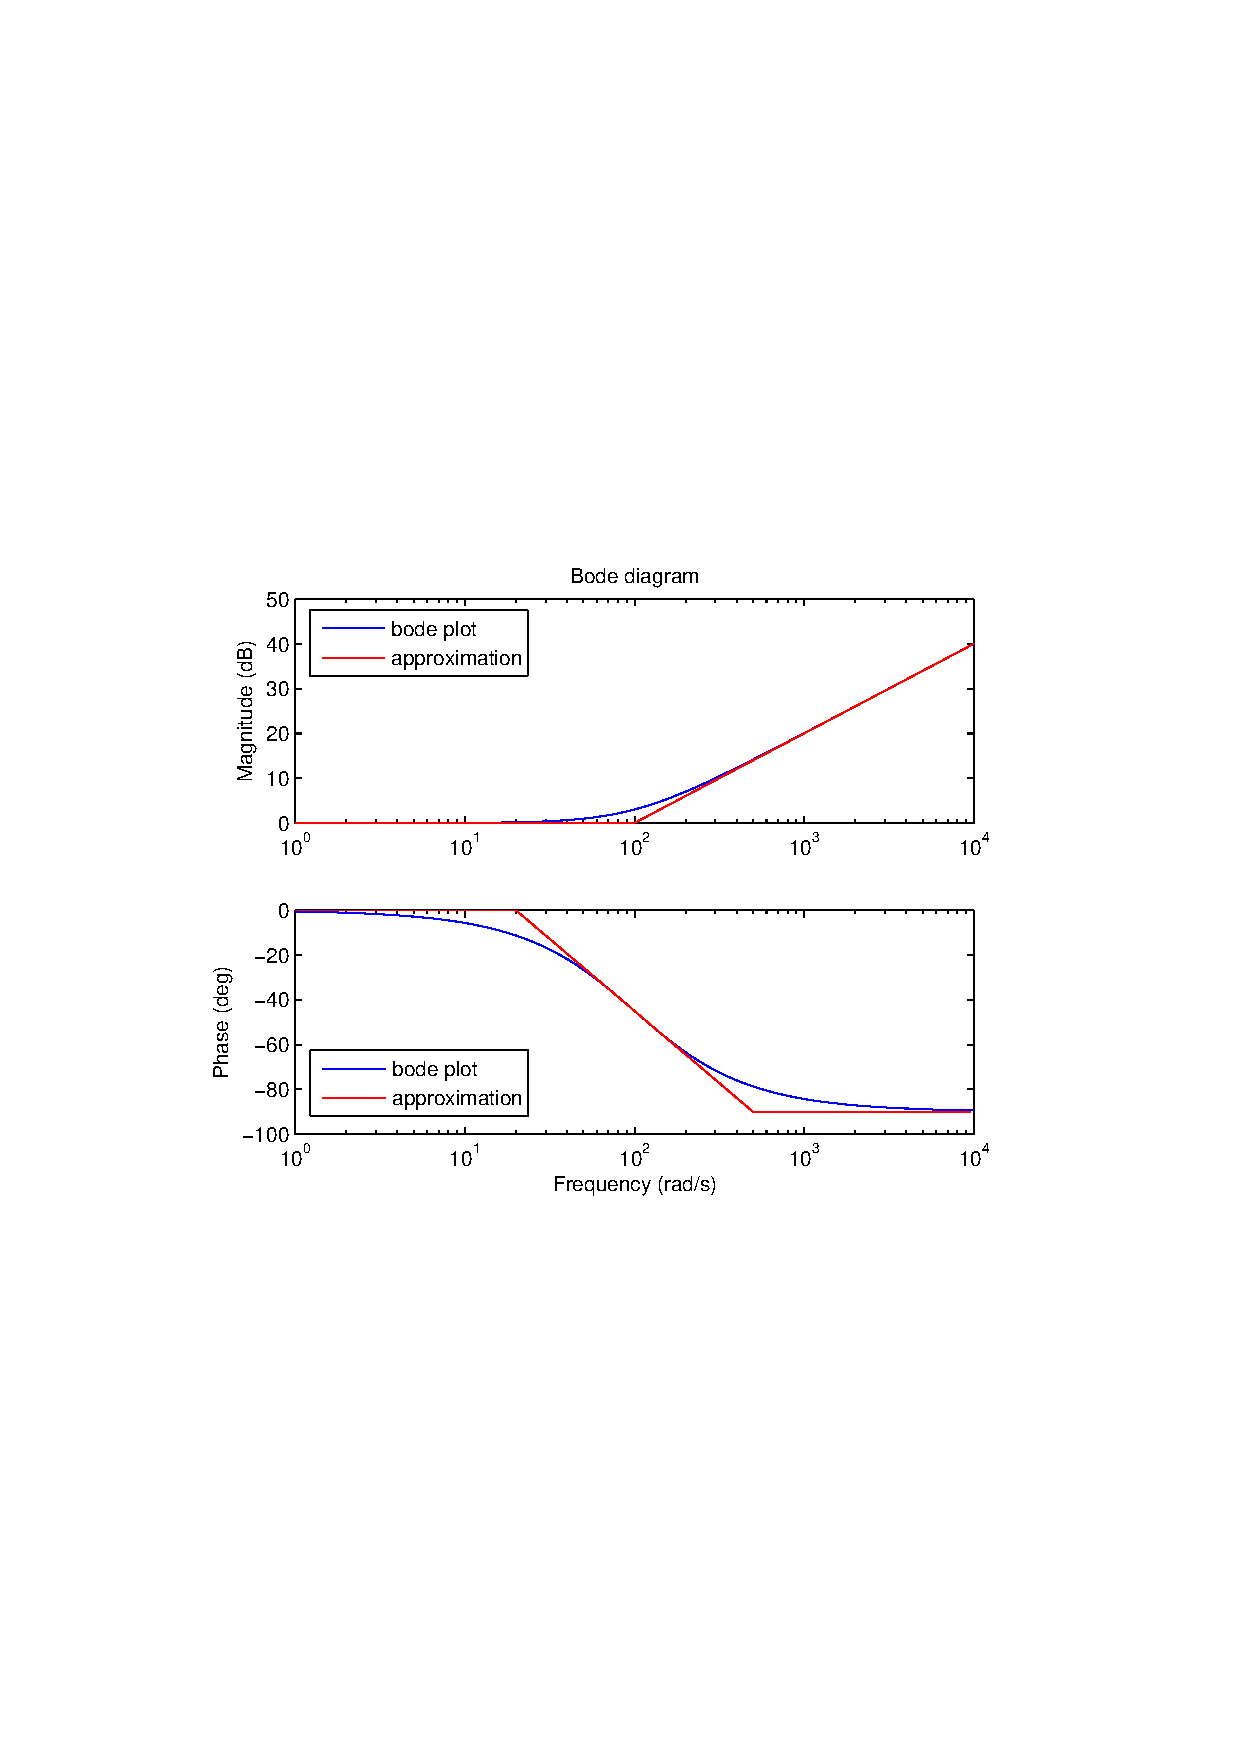
\includegraphics[scale=0.5]{BodeException}

\end{frame}

\section{Examples}

\begin{frame}
\frametitle{Example}

\end{frame}

\section{Conclusion}

\begin{frame}
\frametitle{Conclusion}

\begin{itemize}
\item Today we revised the basics about (constructing) the bode plot
\item These techniques will be used in later lectures regarding controllers
\item The importance of the bode plot will then also be shown
\end{itemize}

\end{frame}


